\chapter{JVM Overview}
\label{chapter:JVM}
\lhead{ \leftmark }

The Java Virtual Machine (JVM) is a stack-based, hardware agnostic virtual machine that is defined by the Java Virtual Machine Specification \cite{jvms7}.  JVM executable code is defined in terms of portable bytecode \cite[4.10]{jvms7} stored in the class file format.

\section{Class File Structure}

The class file format was originally designed to be a binary storage format for compiled Java code.  Due to this, there is a one to one correspondence between structure in a Java source file and corresponding elements in a class file.  Each class file defines one class, which must extend exactly one other class (the \emph{superclass}), and can implement zero or more \emph{interfaces}.  Each class can contain zero or more \emph{fields} and zero or more \emph{methods}.  Given an input Java source file such as Listing \ref{java-before-compile}, a Java compiler would generate a class file output with bytecode representing method \texttt{add} similar to Listing \ref{bc-after-compile}.

\smallskip

\begin{lstlisting}[language=Java,caption=Java before compilation,label=java-before-compile]
  package test;
  class SomeClass {
    int value;
    int add( int b ) {
      return value + b;
    }
  }
\end{lstlisting}

\smallskip

\begin{lstlisting}[language=jvm-bytecode,caption=Mnemonic pseudocode describing the binary structure of class files,label=bc-after-compile]
  .class test/SomeClass
  .super java/lang/Object
    .field value I
    .method add (I)I 
      aload 0
      getfield test/SomeClass/value I
      iload 1
      iadd
      iret
    .end method
  .end class
\end{lstlisting}

Note that even though no \texttt{extends} declaration was used when declaring the class \texttt{SomeClass}, since every class must extend another class the compiler automatically generates bytecode that extends the base class in the Java object system, \texttt{java.lang.Object}.  All classes, fields, and methods within the JVM are strongly typed with symbolic type descriptors \cite[4.3]{jvms7}.  There are two classifications of types within the JVM: \emph{primitive} and \emph{reference} types.  Primitive types are unboxed numeric types such as \texttt{int} and \texttt{boolean} \cite[2.3]{jvms7}.  Reference types refer to dynamically created instances of a class.  Table \ref{table:type-descriptors} shows the format of the type descriptors that will be used throughout this document.

\begin{table}[htbp]
  \centering
  \begin{tabular}{ | l | l | p{5cm} |}
  \hline
  \textbf{Type} & \textbf{Descriptor} \\ \hline
  int & I \\ \hline
  boolean & Z \\ \hline
  void & V \\ \hline
  classref & L\emph{classname}; \\ \hline
  \end{tabular}
  \caption[Type Descriptors]{Type descriptors for common JVM types \cite[4.3.3]{jvms7}.}
  \label{table:type-descriptors}
\end{table}

\subsection{Field and Method Descriptors}

A field descriptor defines the name and type of a class field.  As shown in line 3 of listing \ref{bc-after-compile}, the \texttt{value} field of the class is defined with the type descriptor \texttt{I}, which table \ref{table:type-descriptors} defines as \texttt{int} (a 32-bit two's-complement integer).

A method descriptor is composed of the type descriptors of its parameters and return type \cite[4.3.3]{jvms7}.  As shown in line 4 of Listing \ref{bc-after-compile}, the method \texttt{add(I)I} takes an \texttt{int} parameter and returns an \texttt{int}.  Example mappings between Java method declarations and the resulting method descriptors are provided in Table \ref{table:method-descriptors}.

\begin{table}[htbp]
  \centering
  \begin{tabular}{ | l | l | p{5cm} |}
  \hline
  \textbf{Java Declaration} & \textbf{Method Descriptor} \\ \hline
  void (int a, int b) & (II)V \\ \hline
  boolean (int a, String b) & (ILjava/lang/String;)Z \\ \hline
  \end{tabular}
  \caption[Method Descriptors]{Method Descriptors.}
  \label{table:method-descriptors}
\end{table}


\section{Data Endpoints}

In place of directly addressable memory, all data transfers within the JVM occur between so-called \emph{data endpoints} \cite{nutter-jax2012}.  Data endpoints are strongly typed memory stores that include: an operand stack, a local variable array, class fields, and class methods.  The flow of data between data endpoints is represented in Figure \ref{fig:data-endpoints}.

\begin{figure}[htbp]
  \centering
    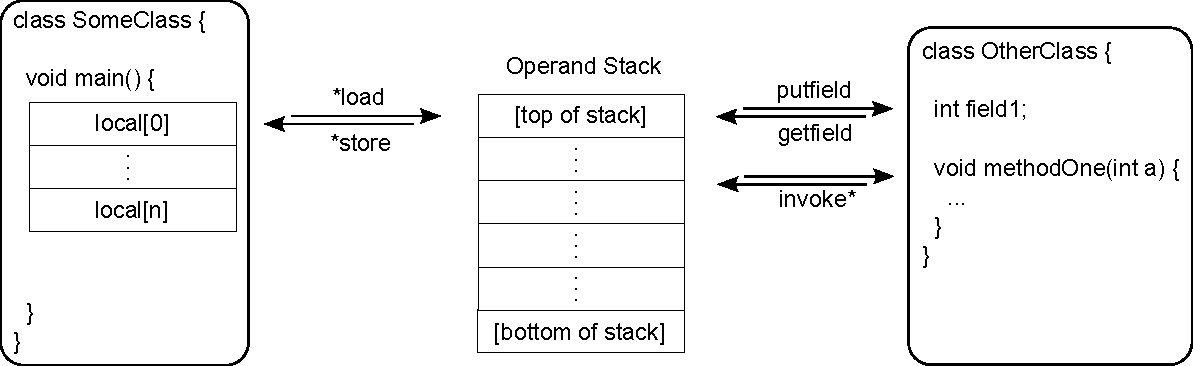
\includegraphics[width=\textwidth]{./Figures/stack-paths.pdf}
  \caption[Data Endpoints]{Data flowing through endpoints.}
	\label{fig:data-endpoints}
\end{figure}

\subsection{Operand Stack}

The \emph{operand stack} is a fixed-sized, Last In First Out (LIFO) data structure \cite[2.6.2]{jvms7} used to perform computation and store intermediary values between other data endpoints.  Each method has access to its own private operand stack during execution, the size of which is determined by the \texttt{maxStack} class file attribute that is specified at compile time.

Values are pushed onto the stack, either explicitly through load instructions or as a result of other instruction execution such as a return value being loaded to the stack after a method invocation.  Once values are on the stack, arithmetic can be performed using instructions like \texttt{iadd} and \texttt{isub} (add and subtract, respectively).  Listing \ref{operand-stack-arithmetic} shows example bytecode that loads values onto the stack and adds them.

\begin{lstlisting}[language=jvm-bytecode,caption=Operand stack arithmetic,label=operand-stack-arithmetic]
  ldc 2  // load constant 2 onto the stack
  ldc 3  // load constant 2 onto the stack
  iadd   // add the top two values on the stack
\end{lstlisting}

\subsection{Local Variables}

During execution, a method has access to a fixed number of local variable slots \cite[2.6.1]{jvms7}.  Listing \ref{locals-java} shows an example Java method that annotates how the locals array is populated.

\begin{lstlisting}[language=Java,caption=Java local variables,label=locals-java]
static int add( int b ) {  // locals[0] = b
  int i = 7;               // locals[1] = i
  int j = 6;               // locals[2] = j
  return b + i + j;
}\end{lstlisting}

Local variables are transferred to and from the operand stack with the \texttt{load} and \texttt{store} opcodes.  Figure \ref{locals-java} shows how the locals array could be allocated given local variable declarations.  Listing \ref{bc-load-store} details how the locals array would interact with the operand stack as depicted in Listing \ref{locals-java} \footnote{Note that compiler optimizations would remove the redundant loads and stores in Listing \ref{bc-load-store}, but it is instructive to retain them.}.

\begin{lstlisting}[language=jvm-bytecode,caption=Load and store,label=bc-load-store]
  ldc 7     // load the constant 7 onto the stack
  istore 1  // store 7 to locals[1]
  ldc 6     // load the constant 6 onto the stack
  istore 2  // store 6 to locals[2]
  iload 0   // load b from locals[0]
  iload 1   // load i from locals[1]
  iload 2   // load j from locals[2]
  iadd      // add i + j
  iadd      // add b to result of i + j
  iret      // return result
\end{lstlisting}

Each load instruction in Listing \ref{bc-load-store} is prefixed by an 'i' to indicate the type of value being loaded.  Integer values require an \texttt{i} prefix, while references require an \texttt{a} prefix.  

The size of the locals array is statically defined within bytecode by the \texttt{maxLocals} attribute of the method.  Attempting to access an index outside of this limit at runtime causes an exception to be thrown.

\subsection{Fields}

Field values of class instances are loaded onto the stack with the \texttt{getfield} instruction and written with the \texttt{putfield} instruction.  Listing \ref{field-java} defines a class \texttt{A} with an integer field \texttt{value} and Listing \ref{bc-getfield} shows the bytecode necessary to read from the \texttt{value} field.

\begin{lstlisting}[language=Java,caption=Java class fields,label=field-java]
package test;
class A {
  int value;
}
\end{lstlisting}

\begin{lstlisting}[language=jvm-bytecode,caption=Load the value of a field onto the stack,label=bc-getfield]
  aload [objectref:A]
  getfield test/A.value I
\end{lstlisting}

After the bytecode in Listing \ref{bc-getfield} executes, the value of the \texttt{value} field of class \texttt{A} will be on the top of the stack.  The bytecode in Listing \ref{bc-putfield} consumes the two values loaded on the stack and sets the value of the \texttt{value} field of class \texttt{A} to 7.

\begin{lstlisting}[language=jvm-bytecode,caption=Set the value of a field,label=bc-putfield]
  aload [objectref:A]
  ldc 7
  putfield test/A.value I
\end{lstlisting}

Access to static fields is performed with the \texttt{getstatic} and \texttt{putstatic} instructions, which behave identically to \texttt{getfield} and \texttt{putfield} except they do not require an object reference to be loaded onto the stack.

\subsection{Method Invocation}

Method invocation is performed by pushing arguments onto the operand stack, then using one of the invocation instructions.  Invocation instructions pop all arguments off the operand stack, including the object reference if present, and push the return value if one exists for the target method.  Each invocation instruction is referred to as a \emph{call site}, and the object reference the method is being called on is referred to as the \emph{receiver}.  Listing \ref{method-java} shows different forms of declared methods in Java source, and Figure \ref{fig:invoke-src-to-bc} shows Java invocations of those methods and the corresponding invocation bytecode.

\begin{lstlisting}[language=Java,caption=Java class methods,label=method-java]
package test;
class A {
  static int a() { ... }
  int b() { ... }
  int c(int i) { ... }
}
\end{lstlisting}

\begin{figure}[htbp]

\begin{minipage}[t]{0.45\textwidth}
\begin{lstlisting}[language=Java,frame=tlrb]
a();
obj.b();

obj.c(9);
\end{lstlisting}
\end{minipage}
\hspace{0.5cm}
\begin{minipage}[t]{0.45\textwidth}
\begin{lstlisting}[language=jvm-bytecode,frame=tlrb]
invokestatic test/A.a ()I
aload [obj]
invokevirtual test/A.b ()I
aload [obj]
ldc 9
invokevirtual test/A.c (I)I
\end{lstlisting}
\end{minipage}

\caption[Invocation Bytecode]{Mapping Java source to bytecode}
\label{fig:invoke-src-to-bc}
\end{figure}

The simplest form of invocation is a static method invocation using the \texttt{invokestatic} instruction, which requires just arguments and a symbolic link to the target method as shown on line 1 of Figure \ref{fig:invoke-src-to-bc}.  Virtual methods (methods declared without the \texttt{static} keyword), are called with the \texttt{invokevirtual} instruction, which requires the object reference of the receiver be pushed on the stack along with the arguments.  If the receiver is an interface, the \texttt{invokeinterface} instruction must be used as shown in Listings \ref{java-interface-decl} and \ref{bc-interface-invoke}.

\begin{lstlisting}[language=Java,caption=Java interface declaration,label=java-interface-decl]
package test;
interface Testable {
  void test(String s);
}
class SomeClass implements Testable {
  void test(String s) { ... }
}
\end{lstlisting}
\vspace{2em}
\begin{lstlisting}[language=jvm-bytecode,caption=Java interface invocation,label=bc-interface-invoke]
invokeinterface test/Testable test (Ljava/lang/String;)V
\end{lstlisting}

If \texttt{invokeinterface} is used with an object reference that does not implement the specified interface, a \texttt{ClassVerifyException} is thrown by the JVM at runtime.

More details about the invocation bytecode instructions can be found in Bill Venner's 1997 JavaWorld article \cite{venners-invocation}.

\section{Bytecode Verification}

All data endpoint access instructions embed not only the symbolic link to their target, but also the target's type descriptor.  Additionally, instructions generally require that a specific combination of operands with specific types are loaded onto the stack in order for them to execute without error.  After the class is loaded into memory and parsed, and before it is made available for execution to other classes within the JVM, the class is run through a verification process to statically prove each instruction has been provided its required operands in the correct order.  Any deviations from the required contract throw a \texttt{ClassVerifyException} at runtime.

\section{Generalization}

All data endpoint access discussed in this chapter goes through the same process: verify permissions, verify target type, verify operand types, and lookup receiver.  The field access instructions can be modeled as function, as shown in Table \ref{table:field-instruction-descriptors}, where \texttt{T} is the field type and \texttt{R} is the receiver type.

\begin{table}[htbp]
  \centering
  \begin{tabular}{ | l | l | p{5cm} |}
  \hline
  \textbf{Instruction} & \textbf{Descriptor} \\ \hline
  \texttt{getfield} & \texttt{(R)T} \\ \hline
  \texttt{putfield} & \texttt{(R,T)V} \\ \hline
  \texttt{getstatic} & \texttt{()T} \\ \hline
  \texttt{putstatic} & \texttt{(T)V} \\ \hline
  \end{tabular}
  \caption[Field Instruction Descriptors]{Field instructions modeled as functions.}
  \label{table:field-instruction-descriptors}
\end{table}

With all data endpoint JVM instructions generalized to function invocations, instructions can be composed at runtime, as Chapter \ref{chapter:Invokedynamic} will discuss in detail.




